\chapter{RELEASE 1}
\addcontentsline{toc}{chapter}{Chapitre 3 : RELEASE 1}

\section*{Introduction}
\addcontentsline{toc}{section}{Introduction}
Après avoir exposé en détail les exigences de notre projet à travers un backlog produit, nous entamons dans ce chapitre la première version du projet, qui comprend deux sprints : le sprint 1 et le sprint 2. Chaque sprint couvre l'analyse, la conception et la réalisation.

\section{Organisation du sprint}
Notre release est composée de deux sprints :\\
\textbf{- Sprint 1 :} Configuration initiale et base du projet.\\
\textbf{- Sprint 2 :} Authentification et gestion des utilisateurs.

\section{Sprint 1 : Configuration initiale et base du projet}
\subsection{Objectif du sprint}
L'objectif de ce sprint est de mettre en place l'environnement MERN, la configuration backend et frontend. Les tâches principales sont :
\begin{itemize}
    \item l'initialisation du dépôt Git ;
    \item la création du serveur Express avec une route de test ;
    \item la modélisation de la base de données MongoDB ;
    \item la configuration de React.js et des routes principales.
\end{itemize}

\section{Sprint 2 : Authentification et gestion des utilisateurs}

\subsection{Objectif du sprint}
L'objectif de ce sprint est de mettre en place un système d'authentification par JWT et une gestion des rôles (participant, gestionnaire, administrateur).  
\textbf{Tâches principales :}
\begin{itemize}
  \item Modélisation \texttt{Utilisateur} avec rôle et état de compte ;
  \item Routes d'inscription, d'authentification et gestion de session (JWT) ;
  \item Interface React pour l'inscription, la connexion et le feedback d'erreur.
\end{itemize}

\subsection{Sprint backlog}
\noindent\textbf{Période :} 12 février – 21 février  
\begin{longtable}{|c|c|m{7cm}|c|c|}
  \caption{User Stories – Sprint 2 : Authentification \& gestion des utilisateurs} \\ \hline
  \textbf{ID} & \textbf{Sprint} & \textbf{User Story} & \textbf{Priorité} & \textbf{Complexité} \\ \hline
  \endfirsthead
  \hline
  \textbf{ID} & \textbf{Sprint} & \textbf{User Story} & \textbf{Priorité} & \textbf{Complexité} \\ \hline
  \endhead
  \hline\endfoot
  \hline\endlastfoot

  \multirow{8}{*}{2} 
  & \multirow{8}{*}{\parbox{3cm}{\centering Authentification et\\ gestion des utilisateurs}} 
  & En tant que participant, je souhaite créer un compte. 
  & Élevée & Moyenne \\ \cline{3-5}
  && En tant que participant, je souhaite me connecter. 
  & Élevée & Moyenne \\ \cline{3-5}
  && En tant que gestionnaire, je souhaite obtenir un compte après validation par l’administrateur. 
  & Élevée & Moyenne \\ \cline{3-5}
  && En tant que gestionnaire, je souhaite me connecter. 
  & Élevée & Moyenne \\ \cline{3-5}
  && En tant qu’administrateur, je veux créer un utilisateur. 
  & Élevée & Moyenne \\ \cline{3-5}
  && En tant qu’administrateur, je veux modifier un utilisateur. 
  & Élevée & Moyenne \\ \cline{3-5}
  && En tant qu’administrateur, je veux supprimer un utilisateur. 
  & Élevée & Moyenne \\ \cline{3-5}
  && En tant qu’administrateur, je veux consulter la liste des utilisateurs. 
  & Élevée & Moyenne \\
  \hline
\end{longtable}

\subsection{Implémentation}

\subsubsection{Politique de création de comptes}
Seuls les \textbf{participants} peuvent créer un compte via le formulaire.  
Les rôles \texttt{gestionnaire} et \texttt{admin} sont créés uniquement par un administrateur qui doit :
\begin{itemize}
  \item recevoir une demande de création (email officiel) ;
  \item vérifier la légitimité du gestionnaire ;
  \item créer manuellement le compte et notifier le gestionnaire.
\end{itemize}

\subsubsection{Spécification des besoins}
On détaille ici trois types de cas d’utilisation :  
\textbf{–} Inscription / Authentification (participant \& gestionnaire)  
\textbf{–} Gestion de comptes (administrateur)  
Chaque cas est accompagné de son diagramme et de sa description textuelle.

\paragraph{Diagramme et description : Inscription \& Authentification}
\begin{figure}[H]
  \centering
  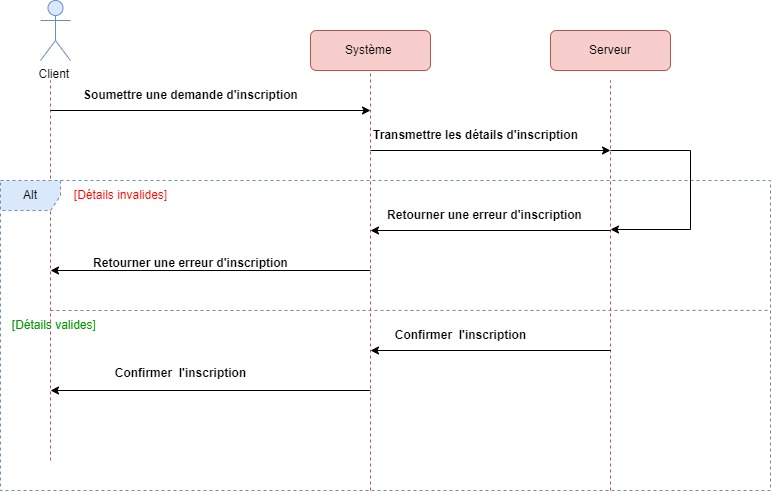
\includegraphics[width=0.6\linewidth]{projet/images/diagramme de sequance/diagrame d'inscription utilisateur.png}
  \caption{Cas d'utilisation « S’inscrire / S’authentifier » (Participant)}
  \label{fig:uc-participant}
\end{figure}

\begin{longtable}{|>{\bfseries}p{4cm}|p{10cm}|}
\hline
Cas d'utilisation & S’inscrire (participant) \\
\hline
Acteur & Participant \\
\hline
Pré-condition & Le formulaire d’inscription est accessible \\
\hline
Post-condition & Compte créé, session ouverte \\
\hline
Scénario principal &
\begin{enumerate}
  \item Affichage du formulaire d’inscription ;
  \item Saisie des informations ;
  \item Soumission et validation ;
  \item Création du compte et feedback de succès.
\end{enumerate} \\
\hline
Scénario alternatif & Email déjà utilisé ou données invalides → message d’erreur \\
\hline
\caption{Inscription participant}
\end{longtable}

\begin{longtable}{|>{\bfseries}p{4cm}|p{10cm}|}
\hline
Cas d'utilisation & S’authentifier (participant \& gestionnaire) \\
\hline
Acteur & Participant / Gestionnaire \\
\hline
Pré-condition & Le compte existe \\
\hline
Post-condition & Token JWT renvoyé, redirection selon rôle \\
\hline
Scénario principal &
\begin{enumerate}
  \item Affichage du formulaire de connexion ;
  \item Saisie des identifiants ;
  \item Soumission, vérification et génération de JWT ;
  \item Stockage du JWT (cookie HTTPOnly).
\end{enumerate} \\
\hline
Scénario alternatif & Identifiants invalides → message d’erreur \\
\hline
\caption{Authentification participant / gestionnaire}
\end{longtable}

\paragraph{Diagramme et description : Gestion des utilisateurs}
\begin{figure}[H]
  \centering
  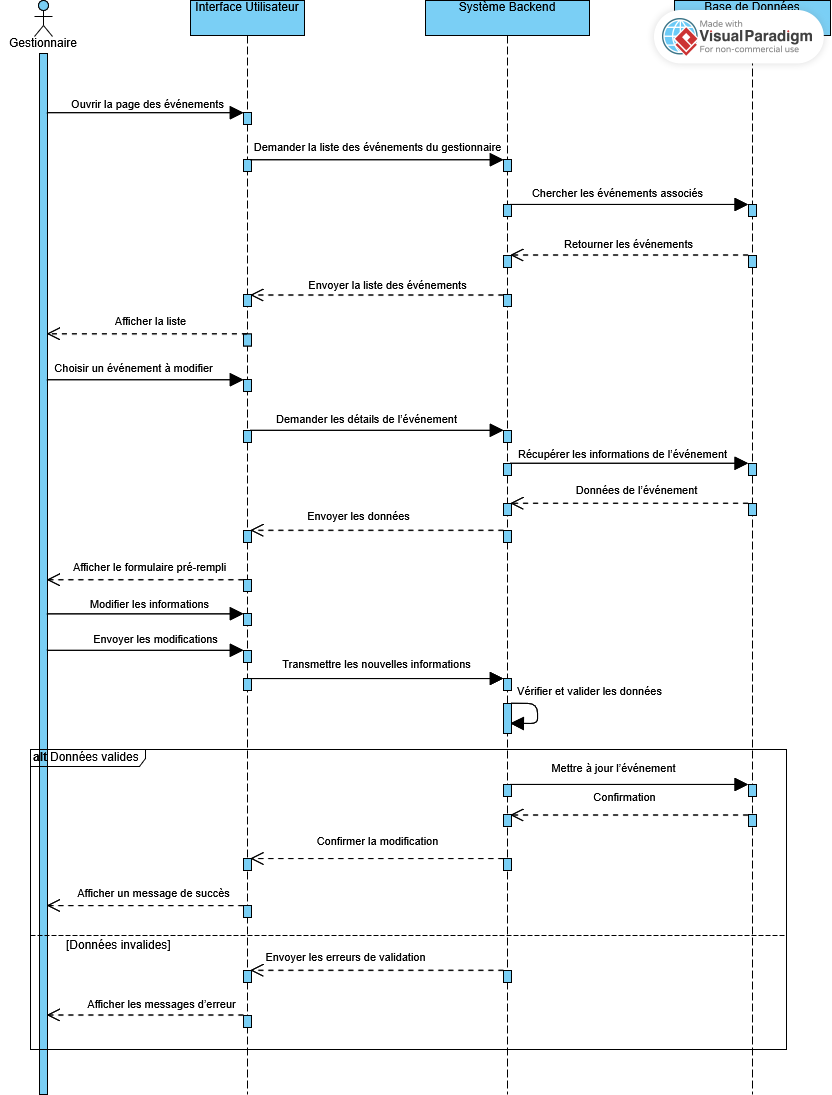
\includegraphics[width=0.6\linewidth]{projet/images/diagramme de sequance/modifier gestionnaire sequance diagram.png}
  \caption{Cas d'utilisation « Gérer les utilisateurs » (Admin)}
  \label{fig:uc-admin}
\end{figure}

\begin{longtable}{|>{\bfseries}p{4cm}|p{10cm}|}
\hline
Cas d'utilisation & Gérer les utilisateurs \\
\hline
Acteur & Administrateur \\
\hline
Pré-condition & Admin connecté \\
\hline
Post-condition & Opération CRUD réalisée \\
\hline
Scénario principal &
\begin{enumerate}
  \item Affichage du tableau des utilisateurs ;
  \item Choix d’une action (Créer, Modifier, Supprimer, Consulter) ;
  \item Exécution de l’opération et feedback.
\end{enumerate} \\
\hline
Scénario alternatif & Erreur de validation ou doublon email → message d’erreur \\
\hline
\caption{Gestion des utilisateurs (Admin)}
\end{longtable}

\subsubsection{Diagrammes de séquence systèmes}
\vspace{-1em}
\begin{figure}[H]
  \centering
  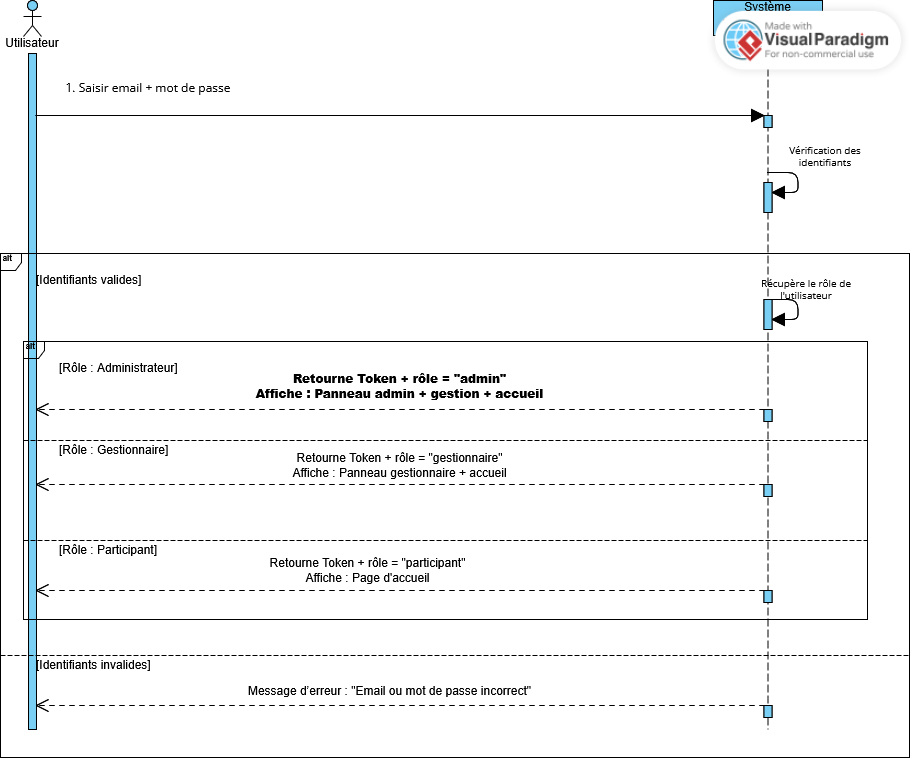
\includegraphics[width=\linewidth]{projet/images/diagramme de sequance/diagrame de sequance s'athentifier.png}
  \caption{Séquence « Authentification / JWT »}
  \label{fig:seq-auth}
\end{figure}

\begin{figure}[H]
  \centering
  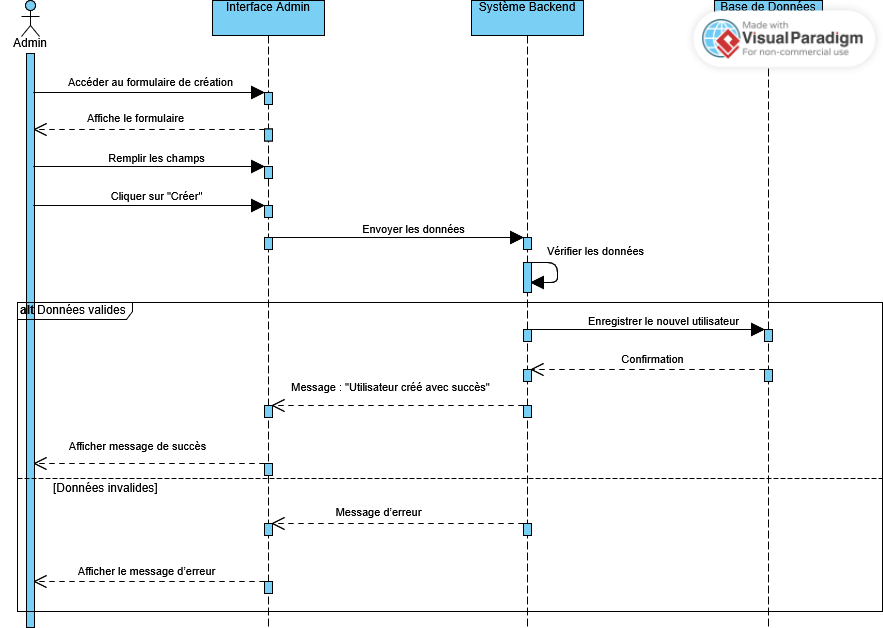
\includegraphics[width=\linewidth]{projet/images/diagramme de sequance/cree utilisateur admin sequance diagram.png}
  \caption{Séquence « CRUD Utilisateurs » (Admin) }
  \label{fig:seq-crud}
\end{figure}

\subsubsection{Diagramme de classe (à compléter)}
% Insérer ici le diagramme de classe Utilisateur / Session / Rôles

\subsubsection{Réalisation}
\noindent\textbf{Formulaires} (inscription / connexion) et \textbf{tableau d’administration} implémentés en React, avec gestion des erreurs et feedback visuel.

\noindent\textbf{Backend} : routes Express sécurisées, génération et vérification de JWT, middleware rôles.

\noindent\textbf{Frontend} : React + Zustand pour l’état d’authentification, Axios pour les requêtes.

